\chapter{Empirical priors: pancreatitis}
\label{applications-priors_empirical}

The GBD 2010 Study often finds that there are a few regions for which detailed data on the
age pattern of disease incidence was available, but many more regions
where incident cases were reported without age-specificity.
Hierarchical modeling using an empirical Bayesian prior is our way to
conduct partial pooling, and borrow strength from the regions with
age-specific data to produce estimates of age patterns in regions
where little or no age-specific data is available.  This chapter shows
the application of empirical priors in estimating sex-specific pancreatitis incidence in
Eastern Europe by borrowing strength from the pooled data.

Pancreatitis is the inflammation of the pancreas, most commonly
caused by alcohol or gallstones.  In most cases, the disease resolves
itself and there is no need for treatment.  However, some acute
cases develop pancreatic necrosis and systemic organ failure.  These
complications require immediate treatment and have a high mortality risk.
\cite{raraty_acute_2004, banks_epidemiology_2002, sekimoto_JPN_2006}

Data from systematic review yielded $3950$ incidence data points, $373$ of which
are from Eastern Europe, the example in this chapter.  As shown in
Figure~\ref{fig:app-pan data}, the data are very heterogeneous and the 
estimates for males and females do not closely

    \begin{figure}[h]
        \begin{center}
            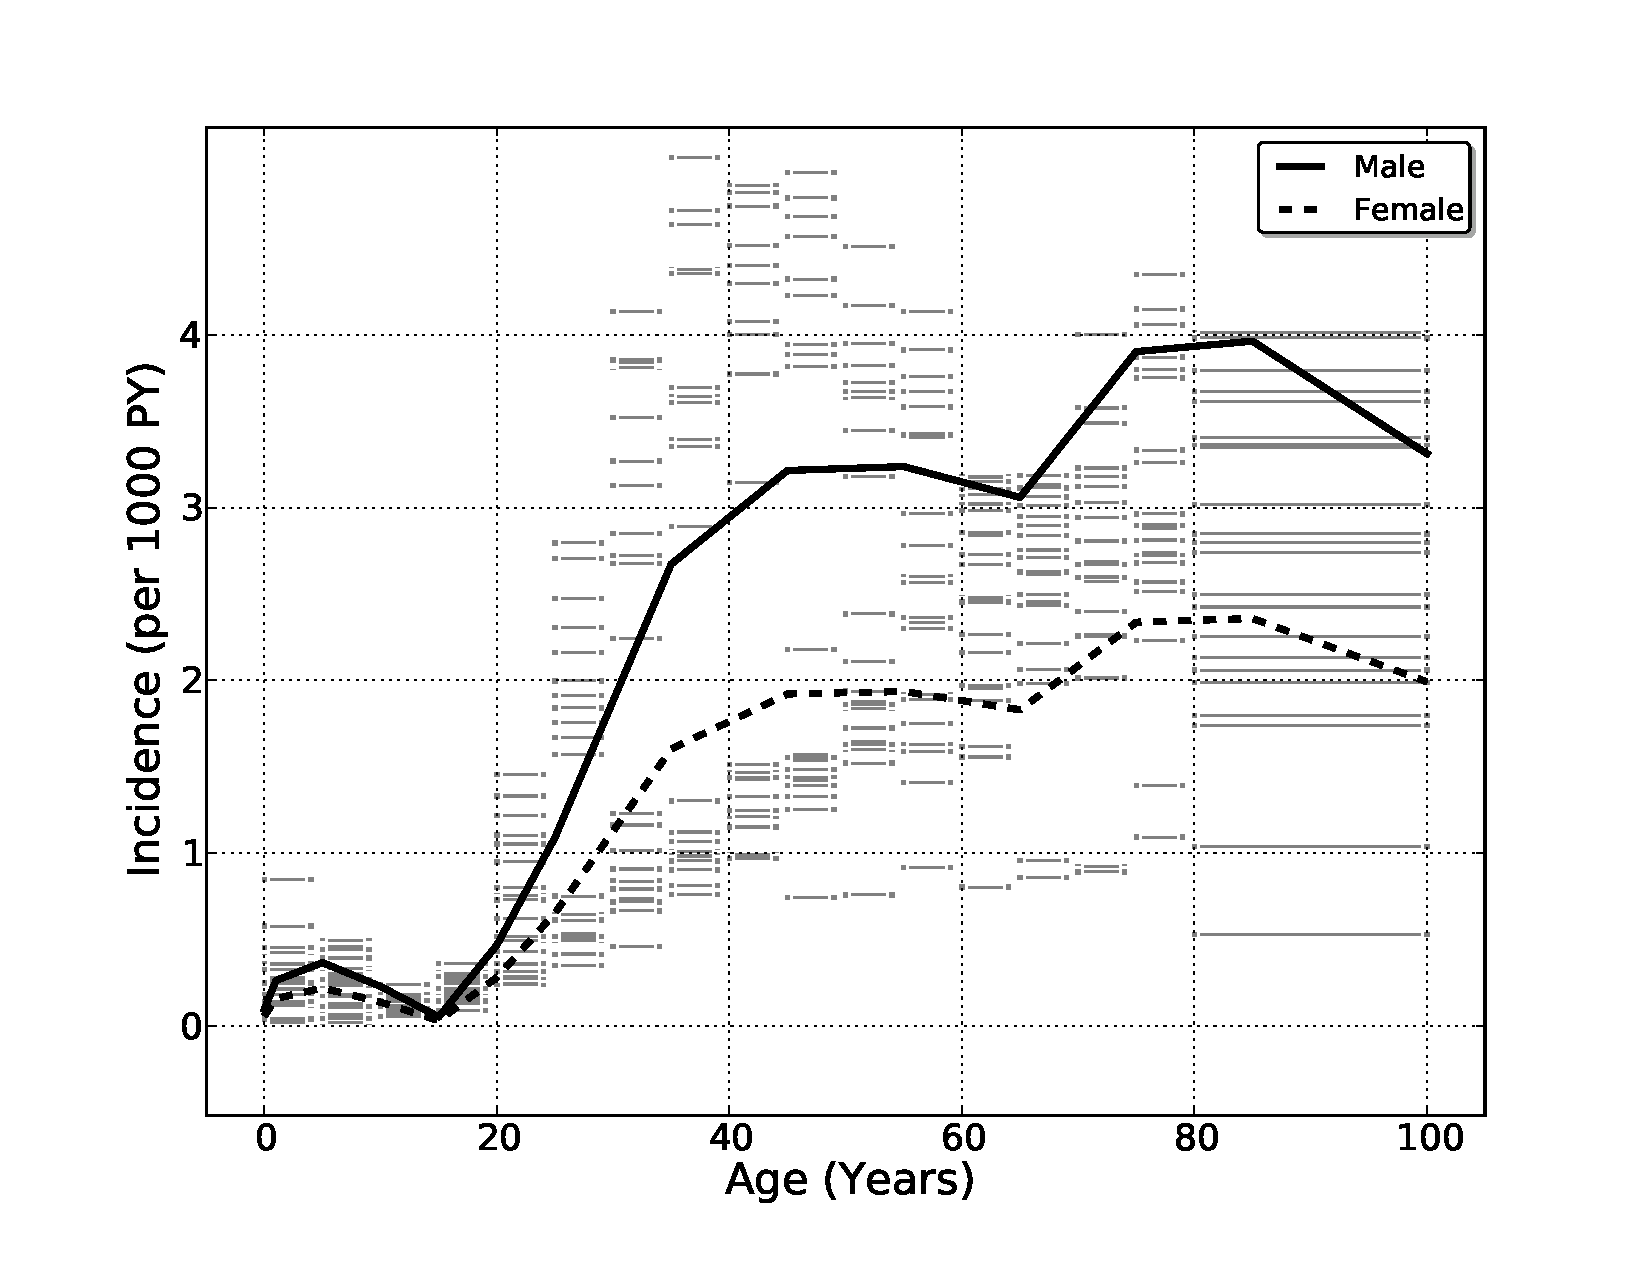
\includegraphics[width=\textwidth]{pancreatitis-data.pdf}
            \caption{Pooled male and female pancreatitis incidence data
              with estimates for males and females in Eastern Europe in 2005.}
            \label{fig:app-pan data}
        \end{center}
    \end{figure}

However, further investigation shows that the data heterogeneity is not
random but the result of a sex differential.  The age-specific incidence
of pancreatitis is very sex-specific.  Using the pooled data estimates from Figure~\ref{fig:app-pan data} as an empirical prior for the sex-specific 
data, the empirical prior updates the estimate as seen in Figure~\ref{fig:app-pan compare}.

    \begin{figure}[h]
        \begin{center}
            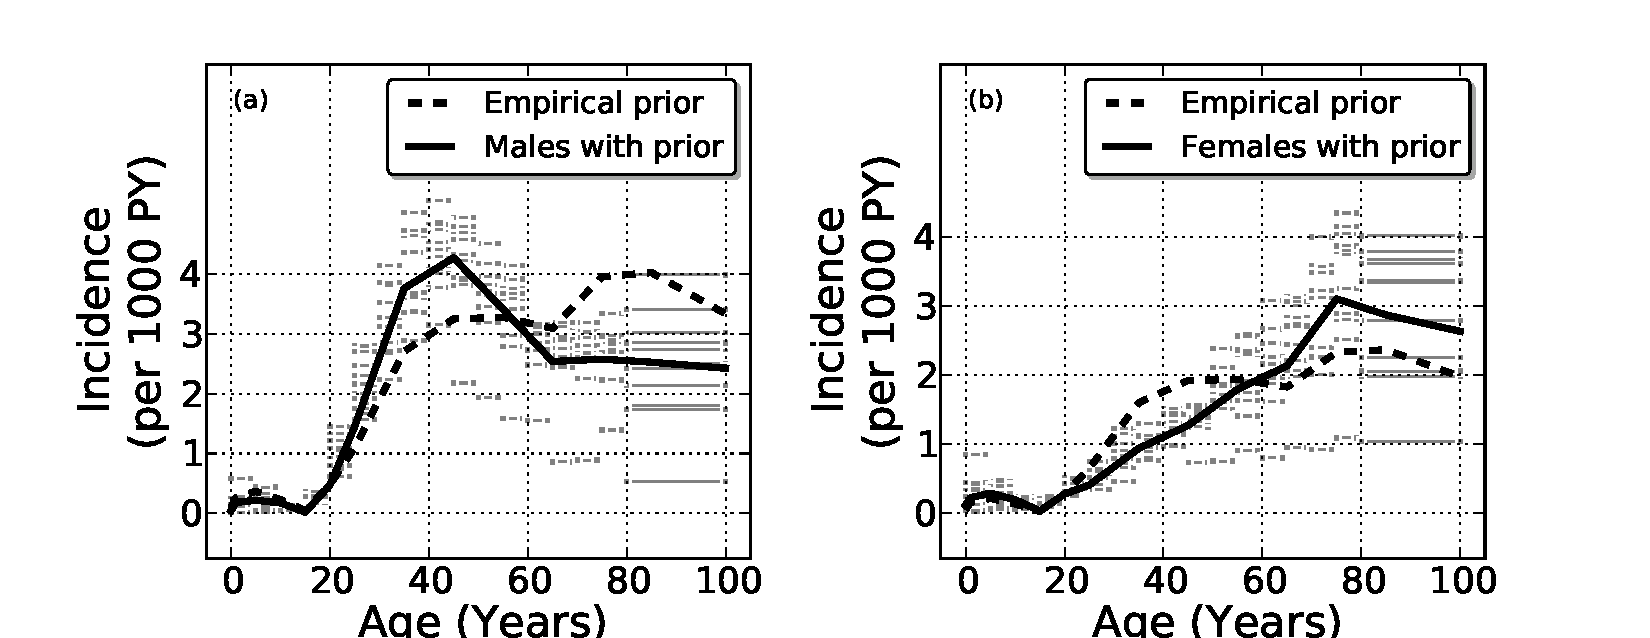
\includegraphics[width=\textwidth]{pancreatitis-compare.pdf}
            \caption{A comparison of incidence estimates for males (a) and
              females (b) in Eastern Europe in 2005.  The estimated incidence 
              using pooled data from Figure~\ref{fig:app-pan data} was applied 
              as an empirical prior to the sex-specific incidence shown to 
              improve estimates.}
            \label{fig:app-pan compare}
        \end{center}
    \end{figure}

Empirical priors provide data-derived relationships to guide the modeling process.
In cases where the data is less clear, empirical priors provide a principled 
way to make less subjective estimates.  